\section{Evaluation}
\label{sec:eval}

In this section, we evaluate the trade-off between the computational performance of a summarisation relation, the volume and the precision of the graph summary.
In this evaluation, we consider the following statements:
\begin{itemize}
	\item $G=\left\langle V, A, l_V \right\rangle$ is a graph;
	\item the bisimulation summary of $G$ is $\mathcal{S}_{fbt} = \left\langle \mathcal{W}_{fbt}, \mathcal{B}_{fbt}, l_{\mathcal{W}_{fbt}} \right\rangle$ according to the summarisation relation $R_{fbt}$;
	\item $\mathcal{S} = \left\langle \mathcal{W}, \mathcal{B}, l_{\mathcal{W}} \right\rangle$ is a summary of $G$ according to the summarisation relation $R$; and
	\item there exists a relation $S \subseteq \mathcal{W}_{fbt} \times \mathcal{W}$ such that $R_{fbt} \sqsubseteq R$.
\end{itemize}

\subsection{Design}

The design of this evaluation is the same as the one describe in Section~\ref{sec:eval:design}. We present here another dimension used for evaluating the precision of the summary.

\begin{quotation}
\item[\emph{Summary precision.}]

With regards to all three classification of errors, we evaluate the precision of a summary thanks to the true and false positive edges set $TP(x)$ and $FP(x)$.
We report the precision using two measures, i.e., $P1$ and $P2$.

The measure $P1$ reflects the average number of true positive edges from a randomly selected node in the inferred graph $\mathfrak{G}(R)$. From right to left, we sum the edge precisions $Prec(R, x)$ of a node $x\in \mathcal{W}_{fbt}$, which we average by the number of nodes within $C(c)$. Finally, we average over the total number of nodes within the bisimulation summary.
$$
\begin{aligned}
P1 = & \frac{1}{\vert \mathcal{W}_{fbt} \vert} \times \sum_{c \in \mathcal{W}}{\frac{1}{\vert C(c) \vert} \times \sum_{x \in C(c)}{Prec(R, x)}} \\
\text{where}\; C(c) = & \left\lbrace x \in \mathcal{W}_{fbt} \mid (x, c) \in S \right\rbrace
\end{aligned}
$$

The measure $P2$ reflects the overall chance for a randomly selected edge in the inferred graph $\mathfrak{G}(R)$ of being a true positive.
$$
P2 = \frac{\sum_{x \in \mathcal{W}_{fbt}}{TP(x)}}{\sum_{x \in \mathcal{W}_{fbt}}{TP(x) + FP(x)}}
$$
\end{quotation}

\subsection{Datasets}

The set of datasets we consider in this evaluation is the same as the one presented in Section~\ref{sec:eval:datasets}.

\subsection{Results}

We evaluate and compare in this section the different graph summary algorithm according to the precision. Then, we discuss the trade-offs with respect to the three dimensions, i.e., the precision we discuss in this section, and the performance and volume dimensions discussed in Section~\ref{sec:summary:eval}.
We note the mean of measurements in a category as $\mu_{L}$, $\mu_{M}$, $\mu_{H}$, and $\mu_{VH}$, respectively.

\subsubsection{Graph Summary Precision}

We discuss in this section the precision of a summary with regards to the connectivity first, then to the type and attribute next. We do not report the precision in any error classification for the \texttt{dbpedia} dataset. The reason is we were unable to evaluate the precision on it due to performance issues. While the performance evaluation did not account for the sumnode $\mathfrak{U}$ of undefined mappings, we do consider it for the precision evaluation.

\minisec{Connectivity Precision}

The Table~\ref{tab:precision-conn} reports the connectivity precision results $P1$ and $P2$. For each category of dataset complexity, we report the mean $\mu$ of the connectivity precision.

The summarisation relations based only on the type feature, i.e., $R_{st}$ and $R_t$, provide a low connectivity precision. Indeed, they show on average a connectivity precision of $25\%$ according to $P1$, i.e., $\mu_H=0.2414$.

Summarisation based on the attribute feature only provide also a low precision on \emph{Medium} and \emph{High} categories. On the \emph{Low} category, the attribute feature exhibits a better precision than the type feature, i.e., $\mu_L=0.5579$ against $\mu_H=0.3617$. However, when the type and attribute features are combined in $R_{at}$, it provides a significant increase of the precision. According to $P1$, we reach on average a $50\%$ connectivity precision ($0.5124$) on the \emph{High} category for $R_{at}$, and at least $20\%$ on \emph{Medium}.

We remark that the incoming attribute in $R_{ioa}$ is an important feature that increases the precision. The $R_{ioa}$ summarisation provides a precision of $30\%$ on the \emph{Medium} up to $50\%$ on \emph{High}, whereas $R_a$ reaches $15\%$ on \emph{Medium} and $10\%$ on \emph{High}. Overall, we can achieve a good average connectivity precision with $R_{ioat}$ according to $P1$. However, the overall precision $P2$ is very low on the datasets of \emph{Medium} and \emph{High} complexities. This suggests that few nodes of the summary have a high out-degree, creating a combinatorial explosion of false positive edges. This will be investigated in future work.

\begin{table}
\centering
\ra{1.2}
\resizebox{\linewidth}{!}{
\begin{tabular}{lc@{\hs}rrc@{\hs}rrc@{\hs}rrc@{\hs}rrc@{\hs}rrc@{\hs}rr}
\toprule
Dataset & \phantom{a} & \multicolumn{2}{c}{$Err(R_{ut})_{con}$} & \phantom{a} & \multicolumn{2}{c}{$Err(R_{t})_{con}$} & \phantom{a} & \multicolumn{2}{c}{$Err(R_{a})_{con}$} & \phantom{a} & \multicolumn{2}{c}{$Err(R_{at})_{con}$} & \phantom{a} & \multicolumn{2}{c}{$Err(R_{ioa})_{con}$} & \phantom{a} & \multicolumn{2}{c}{$Err(R_{ioat})_{con}$} \\
\cmidrule{3-4} \cmidrule{6-7} \cmidrule{9-10} \cmidrule{12-13} \cmidrule{15-16} \cmidrule{18-19}
 & \phantom{a} & $P1$ & $P2$ & \phantom{a} & $P1$ & $P2$ & \phantom{a} & $P1$ & $P2$ & \phantom{a} & $P1$ & $P2$ & \phantom{a} & $P1$ & $P2$ & \phantom{a} & $P1$ & $P2$ \\
%\texttt{dbpedia} & \phantom{a} & - & - & \phantom{a} & 0.0000 & 0.0000 & \phantom{a} & - & -  & \phantom{a} & 0.0000 & 0.0000 & \phantom{a} & - & - & \phantom{a} & 0.0001 & 0.0000 \\
%\midrule
\texttt{twc-logd} & \phantom{a} & 0.0107 & 0.0003 & \phantom{a} & 0.1846 & 0.0002 & \phantom{a} & 0.1444 & 0.0175  & \phantom{a} & 0.5671 & 0.0232 & \phantom{a} & 0.2886 & 0.0222 & \phantom{a} & 0.7572 & 0.0280 \\
\texttt{enipedia} & \phantom{a} & 0.0059 & 0.0005 & \phantom{a} & 0.2982 & 0.0046 & \phantom{a} & 0.0632 & 0.0283  & \phantom{a} & 0.4576 & 0.1047 & \phantom{a} & 0.7294 & 0.1394 & \phantom{a} & 0.9991 & 0.1512 \\
$\mu_H$ & \phantom{a} & \emph{0.0083} & \emph{0.0004} & \phantom{a} & \emph{0.2414} & \emph{0.0024} & \phantom{a} & \emph{0.1038} & \emph{0.0229} & \phantom{a} & \emph{0.5124} & \emph{0.0640} & \phantom{a} & \emph{0.5090} & \emph{0.0808} & \phantom{a} & \emph{0.8781} & \emph{0.0896} \\
\midrule
\texttt{b3kat} & \phantom{a} & 0.3162 & 0.0000 & \phantom{a} & 0.2304 & 0.0000 & \phantom{a} & 0.4975 & 0.0001  & \phantom{a} & 0.5199 & 0.0001 & \phantom{a} & 0.4973 & 0.0001 & \phantom{a} & 0.5217 & 0.0001 \\
\texttt{ecs} & \phantom{a} & 0.0710 & 0.0003 & \phantom{a} & 0.0663 & 0.0002 & \phantom{a} & 0.0145 & 0.0042  & \phantom{a} & 0.0167 & 0.0045 & \phantom{a} & 0.1240 & 0.0070 & \phantom{a} & 0.1030 & 0.0076 \\
\texttt{lobid} & \phantom{a} & 0.0806 & 0.0000 & \phantom{a} & 0.0779 & 0.0001 & \phantom{a} & 0.2480 & 0.0035  & \phantom{a} & 0.3020 & 0.0048 & \phantom{a} & 0.2924 & 0.0072 & \phantom{a} & 0.3483 & 0.0094 \\
\texttt{bnb} & \phantom{a} & 0.0121 & 0.0001 & \phantom{a} & 0.0262 & 0.0001 & \phantom{a} & 0.0091 & 0.0013  & \phantom{a} & 0.0181 & 0.0013 & \phantom{a} & 0.0178 & 0.0013 & \phantom{a} & 0.0299 & 0.0014 \\
\texttt{datos} & \phantom{a} & 0.0206 & 0.0000 & \phantom{a} & 0.0618 & 0.0000 & \phantom{a} & 0.0339 & 0.0000  & \phantom{a} & 0.0653 & 0.0000 & \phantom{a} & 0.1273 & 0.0000 & \phantom{a} & 0.1285 & 0.0000 \\
\texttt{gnd} & \phantom{a} & 0.0086 & 0.0001 & \phantom{a} & 0.0086 & 0.0001 & \phantom{a} & 0.1959 & 0.0091  & \phantom{a} & 0.2158 & 0.0131 & \phantom{a} & 0.6438 & 0.0617 & \phantom{a} & 0.7027 & 0.0880 \\
\texttt{eures} & \phantom{a} & 0.0205 & 0.0018 & \phantom{a} & 0.3617 & 0.0010 & \phantom{a} & 0.1145 & 0.1084  & \phantom{a} & 0.2696 & 0.2227 & \phantom{a} & 0.4833 & 0.3844 & \phantom{a} & 0.4835 & 0.3844 \\
$\mu_M$ & \phantom{a} & \emph{0.0757} & \emph{0.0003} & \phantom{a} & \emph{0.1190} & \emph{0.0002} & \phantom{a} & \emph{0.1591} & \emph{0.0181} & \phantom{a} & \emph{0.2011} & \emph{0.0352} & \phantom{a} & \emph{0.3123} & \emph{0.0660} & \phantom{a} & \emph{0.3311} & \emph{0.0701} \\
\midrule
\texttt{europeana} & \phantom{a} & 0.3641 & 0.0345 & \phantom{a} & 0.3641 & 0.3944 & \phantom{a} & 0.5429 & 0.3944  & \phantom{a} & 0.5429 & 0.3944 & \phantom{a} & 0.5429 & 0.3944 & \phantom{a} & 0.5429 & 0.3944 \\
\texttt{wb} & \phantom{a} & 0.6935 & 0.0476 & \phantom{a} & 0.6320 & 0.0476 & \phantom{a} & 0.9142 & 0.8479  & \phantom{a} & 0.9142 & 0.8479 & \phantom{a} & 0.9680 & 0.9687 & \phantom{a} & 0.9680 & 0.9687 \\
\texttt{cordis} & \phantom{a} & 0.0064 & 0.0094 & \phantom{a} & 0.0064 & 0.0094 & \phantom{a} & 0.1619 & 0.0347  & \phantom{a} & 0.1620 & 0.0347 & \phantom{a} & 0.4203 & 0.0690 & \phantom{a} & 0.4203 & 0.0690 \\
\texttt{ny-times} & \phantom{a} & 0.3830 & 0.0798 & \phantom{a} & 0.3830 & 0.0798 & \phantom{a} & 0.6126 & 0.6813  & \phantom{a} & 0.6126 & 0.6813 & \phantom{a} & 1.0000 & 1.0000 & \phantom{a} & 1.0000 & 1.0000 \\
$\mu_L$ & \phantom{a} & \emph{0.3617} & \emph{0.0428} & \phantom{a} & \emph{0.3464} & \emph{0.1328} & \phantom{a} & \emph{0.5579} & \emph{0.4896} & \phantom{a} & \emph{0.5579} & \emph{0.4896} & \phantom{a} & \emph{0.7328} & \emph{0.6080} & \phantom{a} & \emph{0.7328} & \emph{0.6080} \\
\bottomrule
\end{tabular}
}
\caption{\Gls{connectivity} precision comparison. For each category of dataset complexity, we report the mean $\mu$ of the connectivity precision.}
\label{tab:precision-conn}
\end{table}


\minisec{Schema Precision}

The Table~\ref{tab:precision-schema} reports the means $\mu$ for a category of dataset complexity of the type and attribute precisions results $P1$ and $P2$, i.e., regarding the schema of the summary.

The summarisation $R_{st}$ and $R_t$ based on the type feature provide an attribute precision above at least $60\%$ for $P1$ ($\mu_M=0.5927$ for $\sim_{st}$).
On the contrary, the attribute feature reports a good type precision, reaching on average at least $90\%$ for $R_a$, i.e., $P1=0.9222$ on the \emph{Medium} datasets.

Incoming attributes do not increase much the type precision, since the type precision of $R_a$ stays on par with $R_{ioa}$. The $R_{at}$ relation provides a perfect summarisation of the graph schema. Again, the significant differences between $P1$ and $P2$ suggests one more time that few nodes of the summary contains a high out-degree, creating a combinatorial explosion of false positive edges.\\

\begin{table}
\centering
\ra{1.2}
\resizebox{\linewidth}{!}{
\begin{tabular}{lc@{\hs}rrc@{\s}rrc@{\s}rrc@{\s}rrc@{\s}rrc@{\s}rr}
\toprule
 & \phantom{a} & $P1$ & $P2$ & \phantom{a} & $P1$ & $P2$ & \phantom{a} & $P1$ & $P2$ & \phantom{a} & $P1$ & $P2$ & \phantom{a} & $P1$ & $P2$ & \phantom{a} & $P1$ & $P2$ \\

 & \phantom{a} & \multicolumn{2}{c}{${Err}^{\sim{st}}_{type}$} & \phantom{a} & \multicolumn{2}{c}{${Err}^{\sim{t}}_{type}$} & \phantom{a} & \multicolumn{2}{c}{${Err}^{\sim{a}}_{type}$} & \phantom{a} & \multicolumn{2}{c}{${Err}^{\sim{at}}_{type}$} & \phantom{a} & \multicolumn{2}{c}{${Err}^{\sim{ioa}}_{type}$} & \phantom{a} & \multicolumn{2}{c}{${Err}^{\sim{ioat}}_{type}$} \\
\cmidrule{3-4} \cmidrule{6-7} \cmidrule{9-10} \cmidrule{12-13} \cmidrule{15-16} \cmidrule{18-19}

%%%%% These are the results when considering the set (and not the powerset)

%$\mu_{VH}$ & \phantom{a} & - & - & \phantom{a} & 1.0000 & 1.0000 & \phantom{a} & - & - & \phantom{a} & 1.0000 & 1.0000 & \phantom{a} & - & - & \phantom{a} & 1.0000 & 1.0000 \\
$\mu_{H}$ & \phantom{a} & 1.0000 & 1.0000 & \phantom{a} & 1.0000 & 1.0000 & \phantom{a} & 0.9675 & 0.1424 & \phantom{a} & 1.0000 & 1.0000 & \phantom{a} & 0.9760 & 0.2151 & \phantom{a} & 1.0000 & 1.0000 \\
$\mu_{M}$ & \phantom{a} & 1.0000 & 1.0000 & \phantom{a} & 1.0000 & 1.0000 & \phantom{a} & 0.9222 & 0.7136 & \phantom{a} & 1.0000 & 1.0000 & \phantom{a} & 0.9415 & 0.7753 & \phantom{a} & 1.0000 & 1.0000 \\
$\mu_{L}$ & \phantom{a} & 1.0000 & 1.0000 & \phantom{a} & 1.0000 & 1.0000 & \phantom{a} & 0.9999 & 0.9995 & \phantom{a} & 1.0000 & 1.0000 & \phantom{a} & 0.9999 & 0.9999 & \phantom{a} & 1.0000 & 1.0000 \\

\midrule

 & \phantom{a} & \multicolumn{2}{c}{${Err}^{\sim{st}}_{attr}$} & \phantom{a} & \multicolumn{2}{c}{${Err}^{\sim{t}}_{attr}$} & \phantom{a} & \multicolumn{2}{c}{${Err}^{\sim{a}}_{attr}$} & \phantom{a} & \multicolumn{2}{c}{${Err}^{\sim{at}}_{attr}$} & \phantom{a} & \multicolumn{2}{c}{${Err}^{\sim{ioa}}_{attr}$} & \phantom{a} & \multicolumn{2}{c}{${Err}^{\sim{ioat}}_{attr}$} \\
 \cmidrule{3-4} \cmidrule{6-7} \cmidrule{9-10} \cmidrule{12-13} \cmidrule{15-16} \cmidrule{18-19}
% & \phantom{a} & $P1$ & $P2$ & \phantom{a} & $P1$ & $P2$ & \phantom{a} & $P1$ & $P2$ & \phantom{a} & $P1$ & $P2$ & \phantom{a} & $P1$ & $P2$ & \phantom{a} & $P1$ & $P2$ \\

%$\mu_{VH}$ & \phantom{a} & - & - & \phantom{a} & 0.9745 & 0.0008 & \phantom{a} & - & - & \phantom{a} & 1.0000 & 1.0000 & \phantom{a} & - & - & \phantom{a} & 1.0000 & 1.0000 \\
$\mu_{H}$ & \phantom{a} & 0.7826 & 0.0843 & \phantom{a} & 0.9446 & 0.2398 & \phantom{a} & 1.0000 & 1.0000 & \phantom{a} & 1.0000 & 1.0000 & \phantom{a} & 1.0000 & 1.0000 & \phantom{a} & 1.0000 & 1.0000 \\
$\mu_{M}$ & \phantom{a} & 0.5927 & 0.2798 & \phantom{a} & 0.6607 & 0.2925 & \phantom{a} & 1.0000 & 1.0000 & \phantom{a} & 1.0000 & 1.0000 & \phantom{a} & 1.0000 & 1.0000 & \phantom{a} & 1.0000 & 1.0000 \\
$\mu_{L}$ & \phantom{a} & 0.7586 & 0.5217 & \phantom{a} & 0.7529 & 0.4968 & \phantom{a} & 1.0000 & 1.0000 & \phantom{a} & 1.0000 & 1.0000 & \phantom{a} & 1.0000 & 1.0000 & \phantom{a} & 1.0000 & 1.0000 \\

%\texttt{dbpedia & $P1$ & \phantom{a & - & - & \phantom{a & - & - & \phantom{a & - & - & \phantom{a & - & - & \phantom{a & - & - & \phantom{a & - & - \\
% & $P2$ & \phantom{a & - & - & \phantom{a & - & - & \phantom{a & - & -  & \phantom{a & - & - & \phantom{a & - & - & \phantom{a & - & - \\
%\midrule
%\texttt{twc-logd & $P1$ & \phantom{a & 0.5476 & 0.4882 & \phantom{a & 1.0000 & 0.9496 & \phantom{a & 0.9593 & 1.0000 & \phantom{a & 1.0000 & 1.0000 & \phantom{a & 0.9666 & 1.0000 & \phantom{a & 1.0000 & 1.0000 \\
% & $P2$ & \phantom{a & 0.0000 & 0.0774 & \phantom{a & 1.0000 & 0.0651 & \phantom{a & 0.0000 & 1.0000 & \phantom{a & 1.0000 & 1.0000 & \phantom{a & 0.0000 & 1.0000 & \phantom{a & 1.0000 & 1.0000 \\
%\texttt{enipedia & $P1$ & \phantom{a & 0.7676 & 0.6367 & \phantom{a & 1.0000 & 0.7425 & \phantom{a & 0.9313 & 1.0000 & \phantom{a & 1.0000 & 1.0000 & \phantom{a & 0.9493 & 1.0000 & \phantom{a & 1.0000 & 1.0000 \\
% & $P2$ & \phantom{a & 0.0000 & 0.0000 & \phantom{a & 1.0000 & 0.0000 & \phantom{a & 0.0000 & 1.0000 & \phantom{a & 1.0000 & 1.0000 & \phantom{a & 0.0000 & 1.0000 & \phantom{a & 1.0000 & 1.0000 \\
%$\mu$ & $P1$ & \phantom{a & \emph{0.6576 & \emph{0.5625 & \phantom{a & \emph{1.0000 & \emph{0.8460 & \phantom{a & \emph{0.9453 & \emph{1.0000 & \phantom{a & \emph{1.0000 & \emph{1.0000 & \phantom{a & \emph{0.9580 & \emph{1.0000 & \phantom{a & \emph{1.0000 & \emph{1.0000} \\
% & $P2$ & \phantom{a & \emph{0.0000 & \emph{0.0387 & \phantom{a & \emph{1.0000 & \emph{0.0325 & \phantom{a & \emph{0.0000 & \emph{1.0000}  & \phantom{a & \emph{1.0000 & \emph{1.0000 & \phantom{a & \emph{0.0000 & \emph{1.0000 & \phantom{a & \emph{1.0000 & \emph{1.0000} \\
%\midrule
%\texttt{b3kat & $P1$ & \phantom{a & 0.1089 & 0.0818 & \phantom{a & 1.0000 & 0.1949 & \phantom{a & 0.7372 & 1.0000 & \phantom{a & 1.0000 & 1.0000 & \phantom{a & 0.7420 & 1.0000 & \phantom{a & 1.0000 & 1.0000 \\
% & $P2$ & \phantom{a & 0.0000 & 0.0000 & \phantom{a & 1.0000 & 0.0000 & \phantom{a & 0.0075 & 1.0000 & \phantom{a & 1.0000 & 1.0000 & \phantom{a & 0.0079 & 1.0000 & \phantom{a & 1.0000 & 1.0000 \\
%\texttt{ecs & $P1$ & \phantom{a & 0.8203 & 0.2175 & \phantom{a & 1.0000 & 0.2892 & \phantom{a & 0.8113 & 1.0000 & \phantom{a & 1.0000 & 1.0000 & \phantom{a & 0.8792 & 1.0000 & \phantom{a & 1.0000 & 1.0000 \\
% & $P2$ & \phantom{a & 0.0031 & 0.0000 & \phantom{a & 1.0000 & 0.0000 & \phantom{a & 0.2109 & 1.0000 & \phantom{a & 1.0000 & 1.0000 & \phantom{a & 0.2150 & 1.0000 & \phantom{a & 1.0000 & 1.0000 \\
%\texttt{lobid & $P1$ & \phantom{a & 0.4338 & 0.4832 & \phantom{a & 1.0000 & 0.6670 & \phantom{a & 0.8872 & 1.0000 & \phantom{a & 1.0000 & 1.0000 & \phantom{a & 0.9105 & 1.0000 & \phantom{a & 1.0000 & 1.0000 \\
% & $P2$ & \phantom{a & 0.2176 & 0.3501 & \phantom{a & 1.0000 & 0.4058 & \phantom{a & 0.5879 & 1.0000 & \phantom{a & 1.0000 & 1.0000 & \phantom{a & 0.6677 & 1.0000 & \phantom{a & 1.0000 & 1.0000 \\
%\texttt{bnb & $P1$ & \phantom{a & 0.8503 & 0.5973 & \phantom{a & 1.0000 & 0.5642 & \phantom{a & 0.9900 & 1.0000 & \phantom{a & 1.0000 & 1.0000 & \phantom{a & 0.9895 & 1.0000 & \phantom{a & 1.0000 & 1.0000 \\
% & $P2$ & \phantom{a & 0.5945 & 0.3829 & \phantom{a & 1.0000 & 0.4954 & \phantom{a & 0.8839 & 1.0000 & \phantom{a & 1.0000 & 1.0000 & \phantom{a & 0.9322 & 1.0000 & \phantom{a & 1.0000 & 1.0000 \\
%\texttt{datos & $P1$ & \phantom{a & 0.8156 & 0.5316 & \phantom{a & 1.0000 & 0.5810 & \phantom{a & 0.9999 & 1.0000 & \phantom{a & 1.0000 & 1.0000 & \phantom{a & 0.9999 & 1.0000 & \phantom{a & 1.0000 & 1.0000 \\
% & $P2$ & \phantom{a & 0.5430 & 0.1868 & \phantom{a & 1.0000 & 0.1997 & \phantom{a & 0.9985 & 1.0000 & \phantom{a & 1.0000 & 1.0000 & \phantom{a & 0.9987 & 1.0000 & \phantom{a & 1.0000 & 1.0000 \\
%\texttt{gnd & $P1$ & \phantom{a & 1.0000 & 0.7183 & \phantom{a & 1.0000 & 0.7183 & \phantom{a & 0.9327 & 1.0000 & \phantom{a & 1.0000 & 1.0000 & \phantom{a & 0.9520 & 1.0000 & \phantom{a & 1.0000 & 1.0000 \\
% & $P2$ & \phantom{a & 1.0000 & 0.2422 & \phantom{a & 1.0000 & 0.2422 & \phantom{a & 0.6558 & 1.0000 & \phantom{a & 1.0000 & 1.0000 & \phantom{a & 0.7302 & 1.0000 & \phantom{a & 1.0000 & 1.0000 \\
%\texttt{eures & $P1$ & \phantom{a & 0.9513 & 0.8240 & \phantom{a & 1.0000 & 0.8634 & \phantom{a & 0.9025 & 1.0000 & \phantom{a & 1.0000 & 1.0000 & \phantom{a & 0.9597 & 1.0000 & \phantom{a & 1.0000 & 1.0000 \\
% & $P2$ & \phantom{a & 0.2227 & 0.4629 & \phantom{a & 1.0000 & 0.4658 & \phantom{a & 0.5000 & 1.0000 & \phantom{a & 1.0000 & 1.0000 & \phantom{a & 0.7706 & 1.0000 & \phantom{a & 1.0000 & 1.0000 \\
%$\mu$ & $P1$ & \phantom{a & \emph{0.7114 & \emph{0.4934 & \phantom{a & \emph{1.0000 & \emph{0.5540 & \phantom{a & \emph{0.8944 & \emph{1.0000 & \phantom{a & \emph{1.0000 & \emph{1.0000 & \phantom{a} & \emph{0.9190 & \emph{1.0000} & \phantom{a & \emph{1.0000} & \emph{1.0000} \\
% & $P2$ & \phantom{a & \emph{0.3687 & \emph{0.2321 & \phantom{a & \emph{1.0000 & \emph{0.2584 & \phantom{a & \emph{0.5492 & \emph{1.0000}  & \phantom{a & \emph{1.0000 & \emph{1.0000 & \phantom{a} & \emph{0.6175 & \emph{1.0000} & \phantom{a & \emph{1.0000} & \emph{1.0000} \\
%\midrule
%\texttt{europeana & $P1$ & \phantom{a & 1.0000 & 0.8221 & \phantom{a & 1.0000 & 0.8221 & \phantom{a & 1.0000 & 1.0000 & \phantom{a & 1.0000 & 1.0000 & \phantom{a & 1.0000 & 1.0000 & \phantom{a & 1.0000 & 1.0000 \\
% & $P2$ & \phantom{a & 1.0000 & 0.3823 & \phantom{a & 1.0000 & 0.3823 & \phantom{a & 1.0000 & 1.0000 & \phantom{a & 1.0000 & 1.0000 & \phantom{a & 1.0000 & 1.0000 & \phantom{a & 1.0000 & 1.0000 \\
%\texttt{wb & $P1$ & \phantom{a & 1.0000 & 0.7274 & \phantom{a & 1.0000 & 0.7049 & \phantom{a & 1.0000 & 1.0000 & \phantom{a & 1.0000 & 1.0000 & \phantom{a & 1.0000 & 1.0000 & \phantom{a & 1.0000 & 1.0000 \\
% & $P2$ & \phantom{a & 1.0000 & 0.3856 & \phantom{a & 1.0000 & 0.2863 & \phantom{a & 1.0000 & 1.0000 & \phantom{a & 1.0000 & 1.0000 & \phantom{a & 1.0000 & 1.0000 & \phantom{a & 1.0000 & 1.0000 \\
%\texttt{cordis & $P1$ & \phantom{a & 1.0000 & 0.6922 & \phantom{a & 1.0000 & 0.6922 & \phantom{a & 0.9996 & 1.0000 & \phantom{a & 1.0000 & 1.0000 & \phantom{a & 0.9997 & 1.0000 & \phantom{a & 1.0000 & 1.0000 \\
% & $P2$ & \phantom{a & 1.0000 & 0.6097 & \phantom{a & 1.0000 & 0.6097 & \phantom{a & 0.9956 & 1.0000 & \phantom{a & 1.0000 & 1.0000 & \phantom{a & 0.9991 & 1.0000 & \phantom{a & 1.0000 & 1.0000 \\
%\texttt{ny-times & $P1$ & \phantom{a & 1.0000 & 0.7856 & \phantom{a & 1.0000 & 0.7856 & \phantom{a & 1.0000 & 1.0000 & \phantom{a & 1.0000 & 1.0000 & \phantom{a & 1.0000 & 1.0000 & \phantom{a & 1.0000 & 1.0000 \\
% & $P2$ & \phantom{a & 1.0000 & 0.6933 & \phantom{a & 1.0000 & 0.6933 & \phantom{a & 1.0000 & 1.0000  & \phantom{a & 1.0000 & 1.0000 & \phantom{a & 1.0000 & 1.0000 & \phantom{a & 1.0000 & 1.0000 \\
%$\mu$ & $P1$ & \phantom{a & \emph{1.0000 & \emph{0.7568 & \phantom{a & \emph{1.0000 & \emph{0.7512 & \phantom{a & \emph{0.9999 & \emph{1.0000 & \phantom{a & \emph{1.0000 & \emph{1.0000 & \phantom{a} & \emph{0.9999 & \emph{1.0000 & \phantom{a & \emph{1.0000 & \emph{1.0000} \\
% & $P2$ & \phantom{a & \emph{1.0000 & \emph{0.5177 & \phantom{a & \emph{1.0000 & \emph{0.4929 & \phantom{a & \emph{0.9989 & \emph{1.0000}  & \phantom{a & \emph{1.0000 & \emph{1.0000 & \phantom{a} & \emph{0.9998 & \emph{1.0000 & \phantom{a & \emph{1.0000 & \emph{1.0000} \\
%
%
%%% These are the results with the powerset
%\texttt{dbpedia & \phantom{a & - & - & \phantom{a & - & - & \phantom{a & - & -  & \phantom{a & - & - & \phantom{a & - & - & \phantom{a & - & - \\
%\midrule
%\texttt{twc-logd & \phantom{a & 0.0000 & 0.0774 & \phantom{a & 1.0000 & 0.0651 & \phantom{a & 0.0000 & 1.0000 & \phantom{a & 1.0000 & 1.0000 & \phantom{a & 0.0000 & 1.0000 & \phantom{a & 1.0000 & 1.0000 \\
%\texttt{enipedia & \phantom{a & 0.0000 & 0.0000 & \phantom{a & 1.0000 & 0.0000 & \phantom{a & 0.0000 & 1.0000 & \phantom{a & 1.0000 & 1.0000 & \phantom{a & 0.0000 & 1.0000 & \phantom{a & 1.0000 & 1.0000 \\
%\midrule
%\texttt{b3kat & \phantom{a & 0.0000 & 0.0000 & \phantom{a & 1.0000 & 0.0000 & \phantom{a & 0.0075 & 1.0000 & \phantom{a & 1.0000 & 1.0000 & \phantom{a & 0.0079 & 1.0000 & \phantom{a & 1.0000 & 1.0000 \\
%\texttt{ecs & \phantom{a & 0.0031 & 0.0000 & \phantom{a & 1.0000 & 0.0000 & \phantom{a & 0.2109 & 1.0000 & \phantom{a & 1.0000 & 1.0000 & \phantom{a & 0.2150 & 1.0000 & \phantom{a & 1.0000 & 1.0000 \\
%\texttt{lobid & \phantom{a & 0.0003 & 0.0000 & \phantom{a & 1.0000 & 0.0000 & \phantom{a & 0.0234 & 1.0000 & \phantom{a & 1.0000 & 1.0000 & \phantom{a & 0.0374 & 1.0000 & \phantom{a & 1.0000 & 1.0000 \\
%\texttt{bnb & \phantom{a & 0.1702 & 0.0000 & \phantom{a & 1.0000 & 0.0000 & \phantom{a & 0.0931 & 1.0000 & \phantom{a & 1.0000 & 1.0000 & \phantom{a & 0.7571 & 1.0000 & \phantom{a & 1.0000 & 1.0000 \\
%\texttt{datos & \phantom{a & 0.0449 & 0.0000 & \phantom{a & 1.0000 & 0.0000 & \phantom{a & 0.9922 & 1.0000 & \phantom{a & 1.0000 & 1.0000 & \phantom{a & 0.9945 & 1.0000 & \phantom{a & 1.0000 & 1.0000 \\
%\texttt{gnd & \phantom{a & 1.0000 & 0.0000 & \phantom{a & 1.0000 & 0.0000 & \phantom{a & 0.3230 & 1.0000 & \phantom{a & 1.0000 & 1.0000 & \phantom{a & 0.3904 & 1.0000 & \phantom{a & 1.0000 & 1.0000 \\
%\texttt{eures & \phantom{a & 0.0001 & 0.0000 & \phantom{a & 1.0000 & 0.0000 & \phantom{a & 0.0133 & 1.0000 & \phantom{a & 1.0000 & 1.0000 & \phantom{a & 0.2008 & 1.0000 & \phantom{a & 1.0000 & 1.0000 \\
%\midrule
%\texttt{europeana & \phantom{a & 1.0000 & 0.0000 & \phantom{a & 1.0000 & 0.0000 & \phantom{a & 1.0000 & 1.0000 & \phantom{a & 1.0000 & 1.0000 & \phantom{a & 1.0000 & 1.0000 & \phantom{a & 1.0000 & 1.0000 \\
%\texttt{wb & \phantom{a & 1.0000 & 0.0000 & \phantom{a & 1.0000 & 0.0000 & \phantom{a & 1.0000 & 1.0000 & \phantom{a & 1.0000 & 1.0000 & \phantom{a & 1.0000 & 1.0000 & \phantom{a & 1.0000 & 1.0000 \\
%\texttt{cordis & \phantom{a & 1.0000 & 0.0015 & \phantom{a & 1.0000 & 0.0015 & \phantom{a & 0.9868 & 1.0000 & \phantom{a & 1.0000 & 1.0000 & \phantom{a & 0.9982 & 1.0000 & \phantom{a & 1.0000 & 1.0000 \\
%\texttt{ny-times & \phantom{a & 1.0000 & 0.0607 & \phantom{a & 1.0000 & 0.0015 & \phantom{a & 1.0000 & 1.0000  & \phantom{a & 1.0000 & 1.0000 & \phantom{a & 1.0000 & 1.0000 & \phantom{a & 1.0000 & 1.0000 \\
\bottomrule
\end{tabular}
}
\caption{\gls{schema} precision comparison.}
\label{tab:precision-schema}
\end{table}


In conclusion, we observe that a combination of both type and attribute features is necessary to achieve a good precision. The results show that taking incoming attributes as a feature of the summarisation relation is important for the connectivity precision, but not for the schema.

However, there is place for improvement for overall connectivity precision especially on certain datasets. We observe that the precision $P2$ leads to very low precision values which is caused by a few summary nodes with a high out-degree. This indicates that the model of $P2$ is not appropriate for measuring the precision of a summary in terms of connectivity and schema.

\subsubsection{Trade-Offs}

We report in Figure~\ref{fig:trade-conn-volume} the trade-off between the average connectivity precision and the average volume ratio across all datasets among all the relations. We can distinguish two groups of relations, the type-based summarisations, i.e., $R_t$ and $R_{st}$, and the attribute-based ones.
The type-based relations provide the best volume ratio, but also the worst precision. In the attribute group, the volume ratio among relations is close to each others, but their precision differs greatly, with $R_{ioat}$ ahead. This suggests that in terms of trade-off between connectivity precision and volume, $R_{ioat}$ is the best candidate.

We report in Figure~\ref{fig:trade-schema-volume} the trade-off between the average schema precision and the average volume ratio across all datasets among all the relations. Again we can distinguish the same two groups. However, in the attribute group, the precision does not differ too much among the candidates, each one being either equal or very close to $1$. In the type group, the \emph{Types} summarisation relation $R_t$ provides a quite reasonable precision for a very small volume ratio. This suggests that if the precision is primordial, the \emph{Attributes \& Types} relation $R_{at}$ is the best candidate, providing a perfect schema precision for the smallest volume. However, if volume is primordial instead and that some imperfection can be tolerated, then the \emph{Types} summarisation relation $R_t$ is the best candidate.

We report in Figure~\ref{fig:trade-conn-cpu} (resp., \ref{fig:trade-schema-cpu}) the trade-off between the average connectivity precision (resp., average schema precision) and the average CPU time across all datasets among all the summarisation relations. Among the attribute-based algorithms $R_a$, $R_{at}$, $R_{ioa}$ and $R_{ioat}$, the latter is the one that achieves the best runtime with the highest precision. Among the type-based algorithms, the \emph{Types} summarisation $R_t$ achieves a lower runtime and a higher precision than the \emph{Single-Type} relation $R_{st}$.
If the schema precision is primordial and a low connectivity precision can be tolerated, the \emph{Types} summarisation $R_t$ is the best candidate as it provides a high schema precision, with the best CPU time. On the contrary, if the connectivity is primordial, the summarisation relation $R_{ioat}$ is the best candidate, but this at the cost of a longer runtime.

\begin{figure}
	\centering
	\begin{subfigure}[t]{0.46\textwidth}
		\resizebox{\textwidth}{!}{
			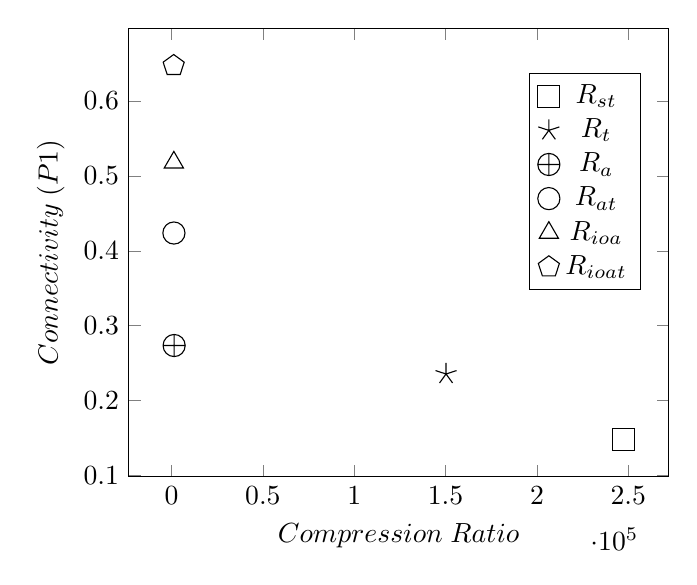
\begin{tikzpicture}
\begin{axis}[
  scatter/classes={
        a={mark=square},%
        b={mark=star},%
        c={mark=oplus},%
        d={mark=o},%
        e={mark=triangle},%
        f={mark=pentagon}
  },
  ylabel=$Connectivity \; (P1)$,
  xlabel=$Compression \; Ratio$,
  mark options={scale=2},
  legend style={at={(.95,0.9)}}
]
\addplot[scatter,only marks,scatter src=explicit symbolic]
coordinates {
% (6.6441, 0.14856667) [a] %0.1301) [a]
% (6.5291, 0.2356) [b] %0.2057) [b]
% (57.4105, 0.2736) [c] %0.2664) [c]
% (65.8846, 0.4238) [d] %0.4221) [d]
% (69.0500, 0.51803333) [e] %0.5169) [e]
% (77.2328, 0.64733333) [f] %0.6598) [f]

(247305.94, 0.14856667) [a]
(150252.41, 0.2356) [b]
(1433.53, 0.2736) [c]
(1314.50, 0.4238) [d]
(1268.24, 0.51803333) [e]
(1184.26, 0.64733333) [f]

};
\legend{$R_{st}$, $R_{t}$, $R_{a}$, $R_{at}$, $R_{ioa}$, $R_{ioat}$}
\end{axis}
\end{tikzpicture}

		}
		\caption{Connectivity precision versus volume ratio.}
		\label{fig:trade-conn-volume}
	\end{subfigure}
	\qquad
	\begin{subfigure}[t]{0.46\textwidth}
		\resizebox{\textwidth}{!}{
			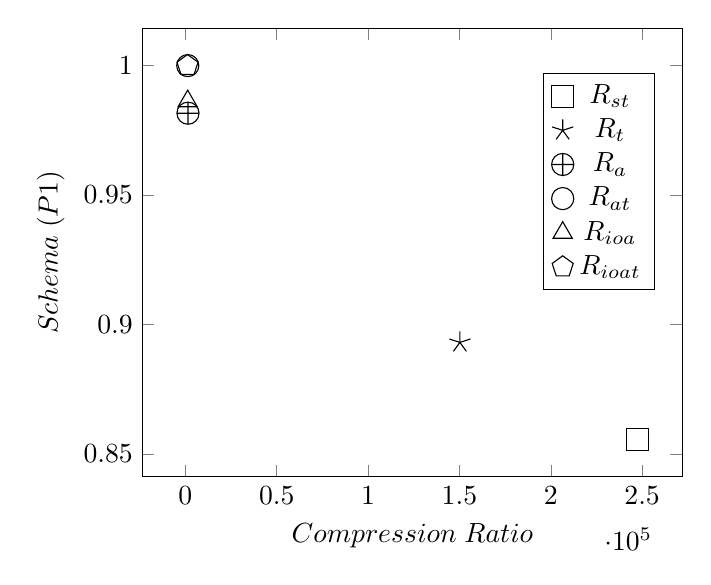
\begin{tikzpicture}
\begin{axis}[
  scatter/classes={
        a={mark=square},%
        b={mark=star},%
        c={mark=oplus},%
        d={mark=o},%
        e={mark=triangle},%
        f={mark=pentagon}
  },
  ylabel=$Schema \; (P1)$,
  xlabel=$Compression \; Ratio$,
  mark options={scale=2},
  legend style={at={(0.95,0.9)}}
]
\addplot[scatter,only marks,scatter src=explicit symbolic]
coordinates {
% (6.6441, 0.85565) [a] %0.6970) [a]
% (6.5291, 0.89303333) [b] %0.8585) [b]
% (57.4105, 0.9816) [c] %0.9733) [c]
% (65.8846, 1.0000) [d]
% (69.0500, 0.98623333) [e] %0.9795) [e]
% (77.2328, 1.0000) [f]

(247305.94, 0.85565) [a]
(150252.41, 0.89303333) [b]
(1433.53, 0.9816) [c]
(1314.50, 1.0000) [d]
(1268.24, 0.98623333) [e]
(1184.26, 1.0000) [f]

};
\legend{$R_{st}$, $R_{t}$, $R_{a}$, $R_{at}$, $R_{ioa}$, $R_{ioat}$}
\end{axis}
\end{tikzpicture}

		}
		\caption{Schema precision versus volume ratio.}
		\label{fig:trade-schema-volume}
	\end{subfigure}
	\qquad%
	\begin{subfigure}[t]{0.46\textwidth}
		\resizebox{\textwidth}{!}{
			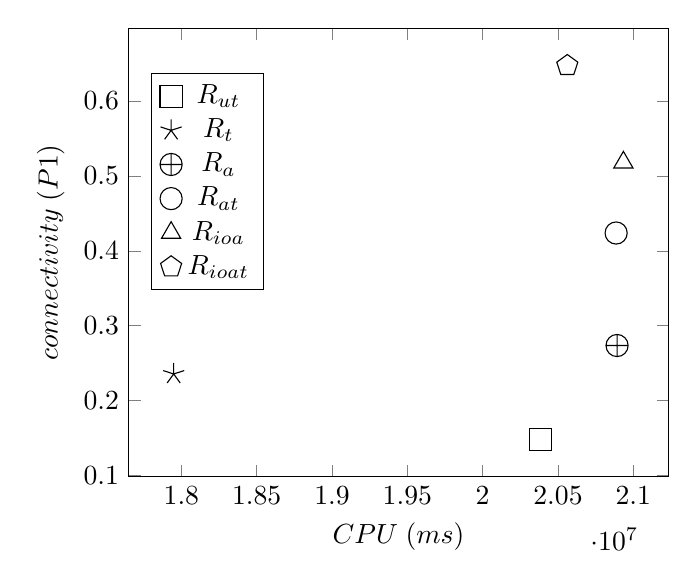
\begin{tikzpicture}
\begin{axis}[
  scatter/classes={
        a={mark=square},%
        b={mark=star},%
        c={mark=oplus},%
        d={mark=o},%
        e={mark=triangle},%
        f={mark=pentagon}
  },
  ylabel=$\gls{connectivity} \; (P1)$,
  xlabel=$CPU \; (ms)$,
  mark options={scale=2},
  legend style={at={(0.25,0.9)}}
]
\addplot[scatter,only marks,scatter src=explicit symbolic]
coordinates {
% (24844125.1190, 0.1301) [a]
% (24669863.0952, 0.2057) [b]
% (24277682.3810, 0.2664) [c]
% (28968841.4286, 0.4221) [d]
% (22053489.7619, 0.5169) [e]
% (22386809.1667, 0.6598) [f]
 (20384066, 0.14856667) [a]
 (17949001, 0.2356) [b]
 (20892062, 0.2736) [c]
 (20885921, 0.4238) [d]
 (20934061, 0.51803333) [e]
 (20561815, 0.64733333) [f]
};
\legend{$R_{ut}$, $R_{t}$, $R_{a}$, $R_{at}$,
 $R_{ioa}$, $R_{ioat}$}
\end{axis}
\end{tikzpicture}

		}
		\caption{Connectivity precision versus summarisation performance.}
		\label{fig:trade-conn-cpu}
	\end{subfigure}
	\qquad%
	\begin{subfigure}[t]{0.46\textwidth}
		\resizebox{\textwidth}{!}{
			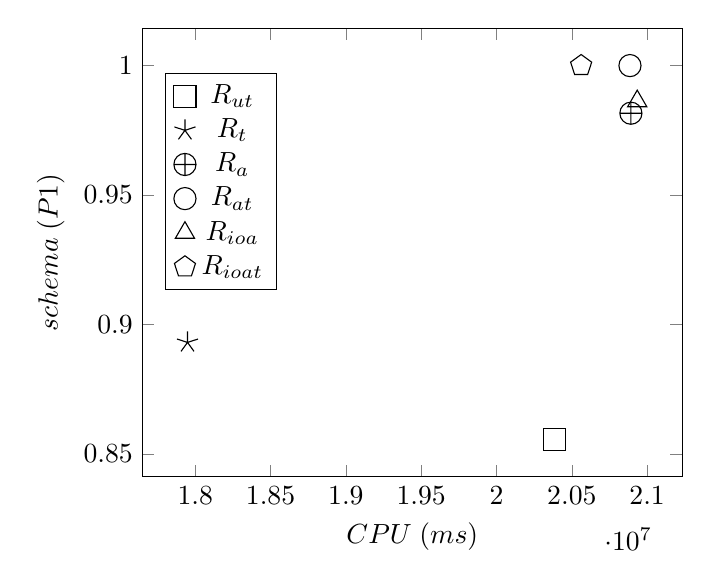
\begin{tikzpicture}
\begin{axis}[
  scatter/classes={
        a={mark=square},%
        b={mark=star},%
        c={mark=oplus},%
        d={mark=o},%
        e={mark=triangle},%
        f={mark=pentagon}
  },
  ylabel=$\gls{schema} \; (P1)$,
  xlabel=$CPU \; (ms)$,
  mark options={scale=2},
  legend style={at={(0.25,0.9)}}
]
\addplot[scatter,only marks,scatter src=explicit symbolic]
coordinates {
% (24844125.1190, 0.6970) [a]
% (24669863.0952, 0.8585) [b]
% (24277682.3810, 0.9733) [c]
%% (28968841.4286, 1.0000) [d]
% (22053489.7619, 0.9795) [e]
% (22386809.1667, 1.0000) [f]

 (20384066, 0.85565) [a]
 (17949001, 0.89303333) [b]
 (20892062, 0.9816) [c]
 (20885921, 1) [d]
 (20934061, 0.98623333) [e]
 (20561815, 1) [f]
};
\legend{$R_{ut}$, $R_{t}$, $R_{a}$, $R_{at}$, $R_{ioa}$, $R_{ioat}$}
\end{axis}
\end{tikzpicture}

		}
		\caption{Schema precision versus summarisation performance.}
		\label{fig:trade-schema-cpu}
	\end{subfigure}
	\caption{Efficiency and precision trade-offs of the candidate summarisation relations. The values are taken as the average across all dataset categories.}
\end{figure}
